\documentclass[
	12pt, % Default font size, values between 10pt-12pt are allowed
	%letterpaper, % Uncomment for US letter paper size
	%spanish, % Uncomment for Spanish
]{fluids_report_style}

\usepackage{my_packages}
\usepackage{comment}
\usepackage[inkscapeformat=png]{svg}
\usepackage{subcaption}
\usepackage{multicol}
\usepackage[hidelinks,colorlinks=true,linkcolor=blue,citecolor=blue]{hyperref}
\usepackage[font=small,labelfont=bf]{caption}

\title{Fluids Poject}        % Assignment title
\author{Heath Buer, Joshua Hoffman, McCade Hughes, Bennet Outland, Joseph Romero}   % Student name
%Partner Name
%\roll{Lorem Ipsum, Lorem Ipsum}                    % Class roll
\class{Thermo Fluid Dynamics}              % Class
\session{M01}             % Session
\email{\\ heath.buer@mines.sdsmt.edu \\ joshua.hoffman@mines.sdsmt.edu \\  lane.hughes@mines.sdsmt.edu \\ bennet.outland@mines.sdsmt.edu \\ joseph.romero@mines.sdsmt.edu}
\date{May 2, 2023}% Due date
\institute{Department of Mechanical Engineering}              % Institute or school name
\course{ME 331}                            % Course or course name
\professor{Dr. John Thalakkottor}                                           % Professor or teacher in charge of the assignment

%------------------------------------------------------------------------------------
\addbibresource{ref.bib} 

\setcounter{secnumdepth}{-2} 
%\renewcommand{\thesection}{}  % https://tex.stackexchange.com/a/30202/114006
%------------------------------------------------------------------------------------
\begin{document}
\maketitle 
\begin{table}
    \centering
    \begin{tabular}{c|c}
        Name & \% Effort \\
        \hline
        Heath Buer & 20\% \\
        Joshua Hoffman & 20\% \\
        McCade Hughes & 20\% \\
        Bennet Outland & 20\% \\
        Joseph Romero & 20\%
    \end{tabular}
\end{table}





\pagenumbering{gobble}  
\newpage
\pdfbookmark[section]{\contentsname}{toc}
\tableofcontents
\newpage
\pagenumbering{arabic}          % to start the page numbering

%-----------------------------------------

%1 
\section{Summary}
In this project, we were tasked with determining the minimum length of a runway and the maximum thrust required for takeoff for a given airplane on an island (sea level). In order to determine this, the Coefficient of Drag ($C_D$) and Coefficient of Lift ($C_L$) need to be found for a given wing geometry. The values for the Coefficient of Lift and Drag for a Clark Y-14 Airfoil at different velocities and angles of attack ($\alpha$) were determined using both a computational fluid dynamics (CFD) simulation and a wind tunnel experiment. This data was used to determine the minimum runway length and maximum thrust required for take-off. As a result, the minimum runway length, with a safety factor of 1.25, was determined to be $4640$ m and the maximum thrust was determined to be $113$ kN. 

%2 
\section{Introduction}
\begin{comment}
The introduction serves as a preparation for the material to follow and relates the current work on the
subject to the field. As much of the following material as is applicable should be included in any logical
order:
1. The status of the problem prior to the present research
2. The purpose of the investigation precisely defined
3. The conditions under which the work was done and the procedure, if unusual
4. The scope of the present work and its connection with the general problem
5. Recognition of similar work on the subject
6. Significance of the material treated
In addition, it may be desirable to state where and when the work was done. Such mention should occur
in the introduction unless it is specifically included in a following section.
\end{comment}

A Clark Y-14 Airfoil is a standard airfoil that has been well-tested. We investigate the properties of this airfoil for educational advancements and validation of previous results. Using a subsonic wind tunnel and a test model for a Clark Y-14 Airfoil, the Coefficient of Lift and Coefficient of Drag were experimentally determined for different velocities and angles of attack. Each experiment was repeated twice to account for the statistical variances in the results. A CFD simulation was also used to determine the Coefficient of Lift and Coefficient of Drag values. The wind tunnel data was used to validate the CFD data. We will compare our airfoil data against literature data, such as the data repository on Airfoil Tools \cite{clark_y_airfoil}. We apply this data to the case of a plane landing on an island where the parameters for the plane were given as follows: mass equal to 45,000 kg with a wingspan of 35m and an aspect ratio of 8. The Coefficient of Drag and Coefficient of Lift values were then used to determine the minimum required runway length for safe take-off and landing as well as the maximum thrust required for take-off. This investigation is vital to ensure safe runway construction.

%3 
\section{Description of Apparatus}
\begin{comment}
For papers presenting experimental data this section is usually a brief but adequate discussion of the appa-
ratus used, the material employed, the models tested, and the experimental setup. Unless the equipment is
new or modified, suitable references to a published description is satisfactory. Dimension and descriptions of
unmodified, permanent equipment should be kept in present tense. Trade names of equipment or material,
including aircraft and engines, may be used, if necessary, for identification and if no evaluation is presented.
Any sketched or photographs of the equipment, setup, and tests in progress should be referred to in this
section.
\end{comment}

One method used to determine the Coefficient of Lift was pressure data from a wind tunnel experiment utilizing an AeroLab wind tunnel. The Clark Y-14 Airfoil was tested in the wind tunnel for velocities ranging from 40mph to 70mph. Pressure data was taken at angles of attack of 0$^\circ$, 5$^\circ$, 10$^\circ$, 15$^\circ$, and 20$^\circ$. The pressure data was taken using 18 small orifices in the airfoil surface connected to an array of manometers. Height differences for each manometer were taken in reference to a manometer connected to the atmosphere. These height differences were used to determine the pressure profile around the airfoil. 

\begin{figure}[H]% 
    \centering
    {{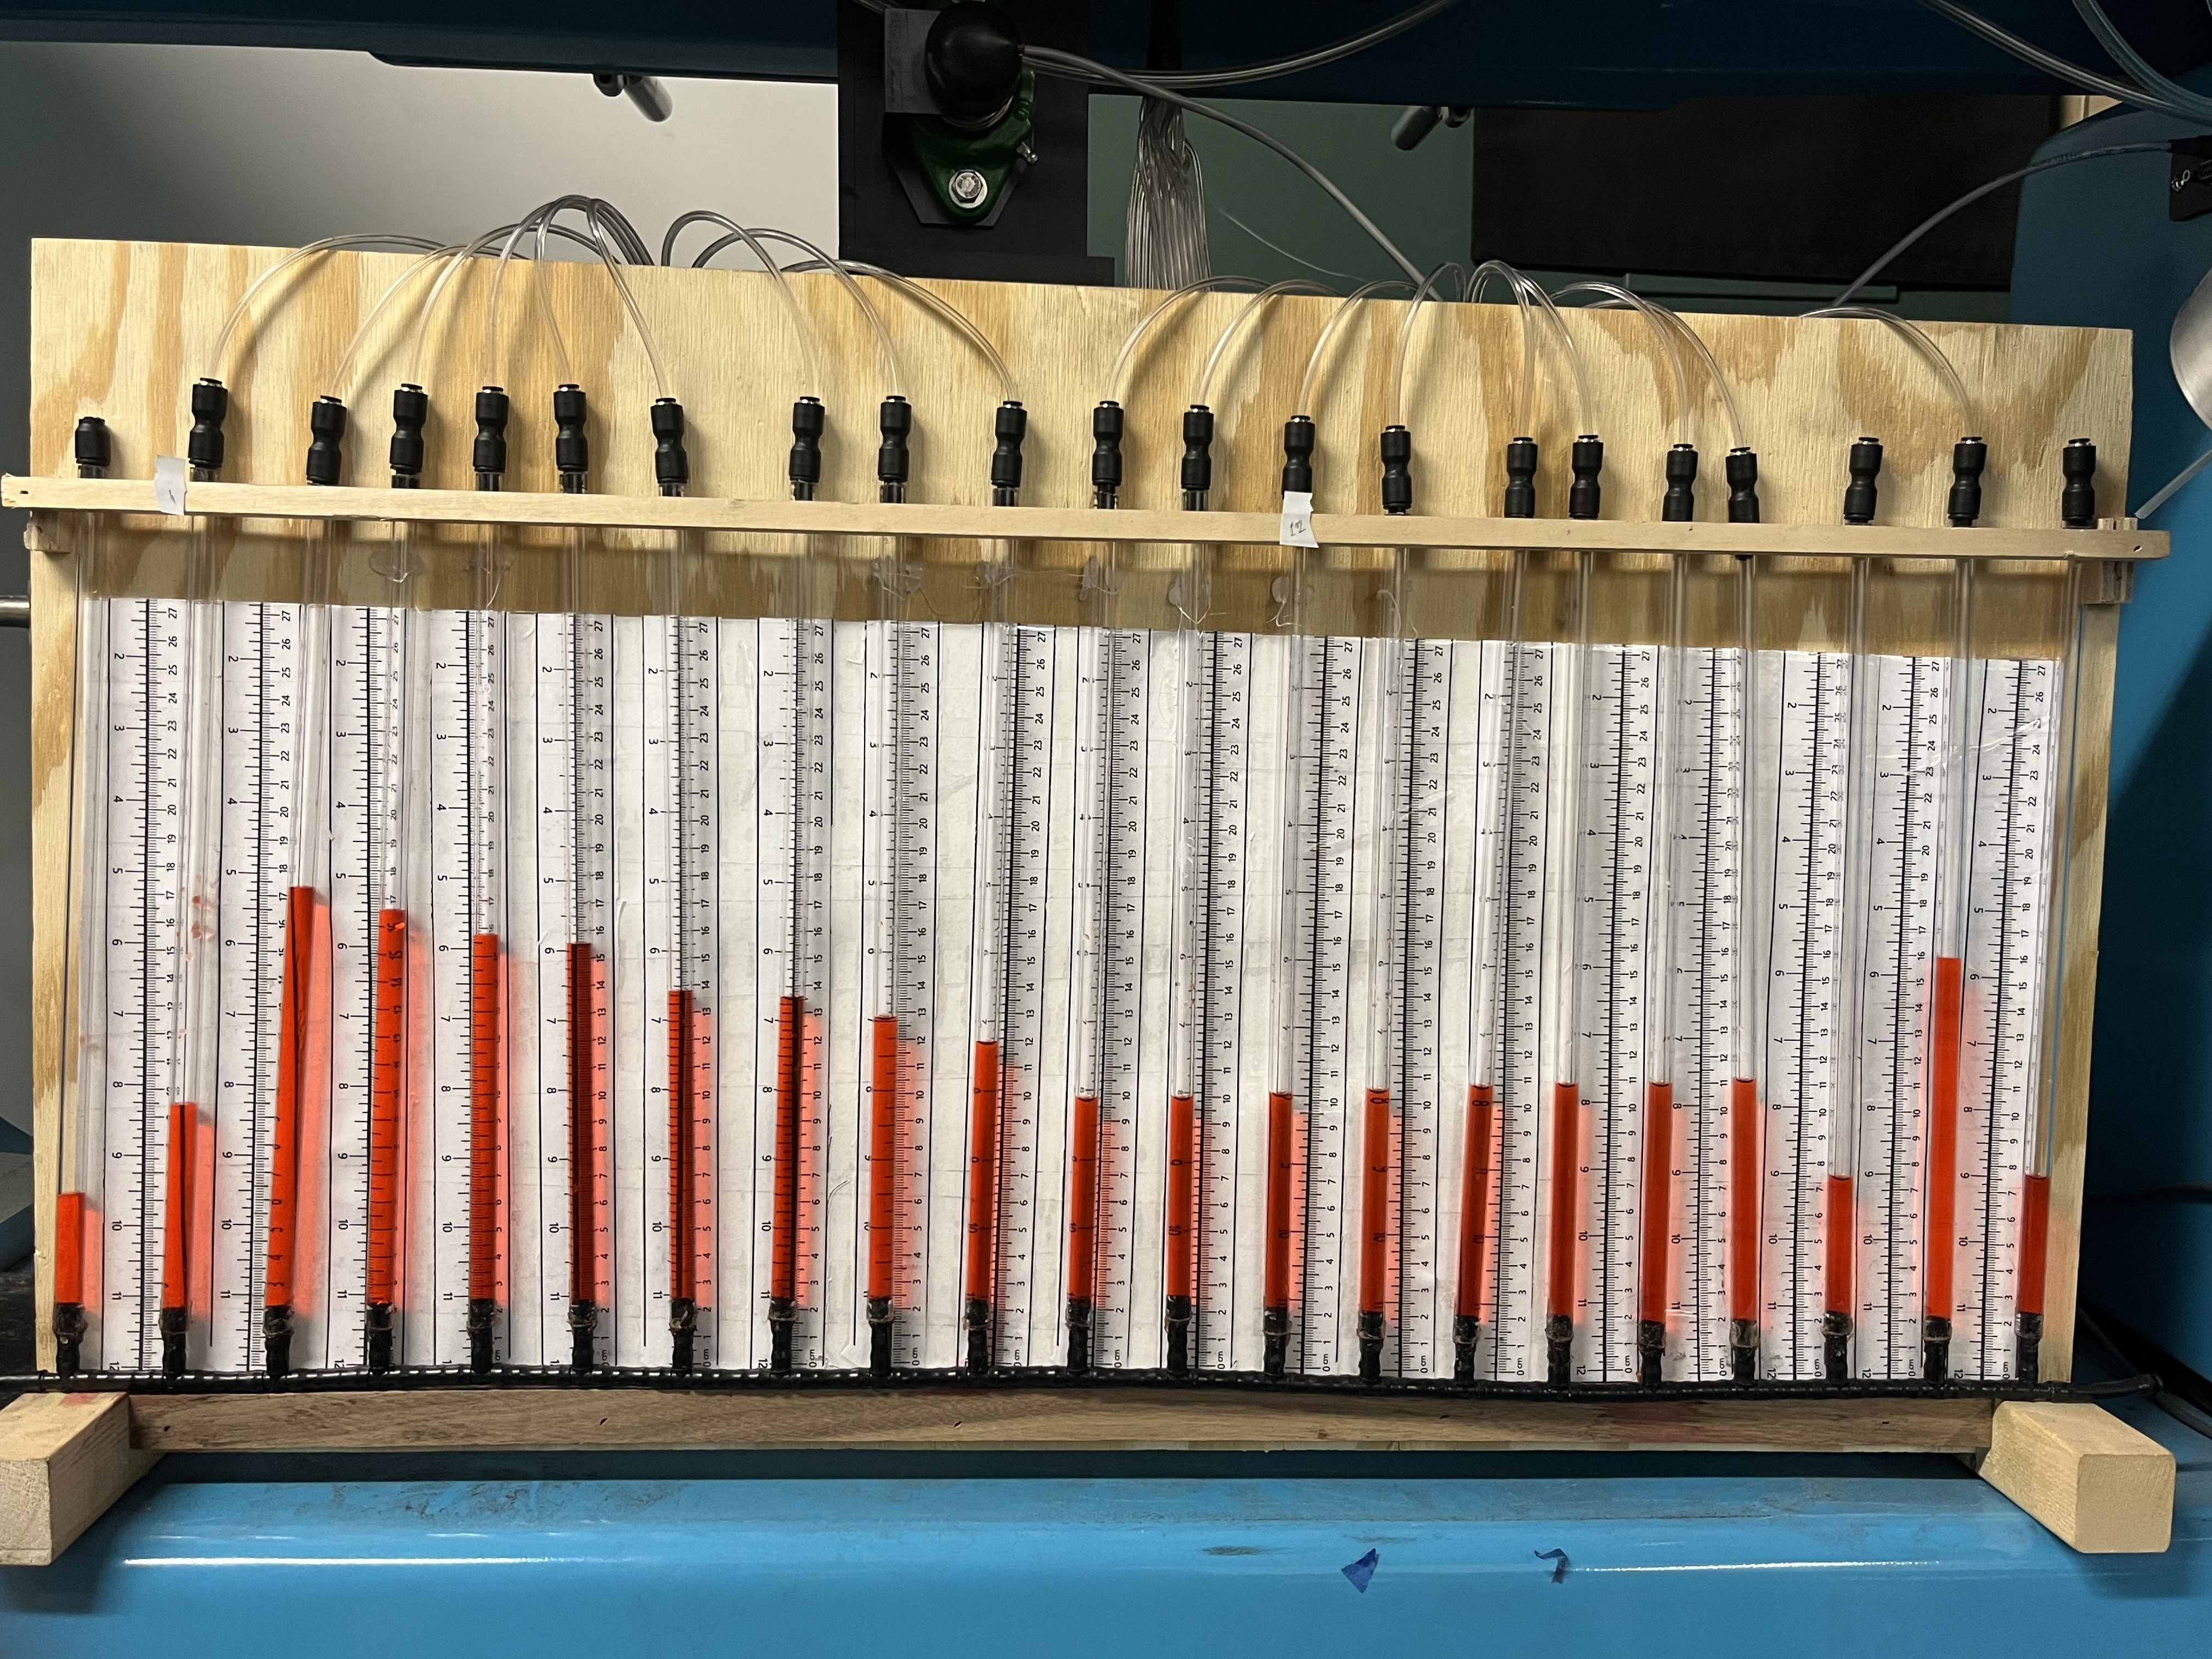
\includegraphics[width=10cm]{figures/IMG_0249.jpg} }}% 
    \caption{Sample image of the manometer array used to determine the pressure profile around the airfoil.}
    \label{fig:manometer}%
\end{figure}  

% Describe the math behind finding C_D and C_L using pressure data (trapezoidal rule etc.). 

%4 
\section{Description of Numerical Simulation} 

The CFD simulation was conducted under the assumption that the flow around the airfoil was laminar. Therefore, the K-epsilon Model in Ansys Fluent \cite{ansys} was used to conduct this simulation. Because this simulation was 2-D, the edges of the geometry were selected to be boundary conditions. The top and bottom edges of the geometry were assigned "symmetry". The left edge was the inlet, the right edge was the outlet, and the airfoil itself was assigned "wall" (see Figure (\ref{fig:BC})). The mesh consisted of linear elements. As a result, the edges and the surface were assigned a mesh size of $5(10^{-3})$ft. At the boundary of the airfoil, the mesh size was $1(10^{-3})$ft (see Figure (\ref{fig:Mesh})). 

\begin{figure}[H]% 
    \centering
    {{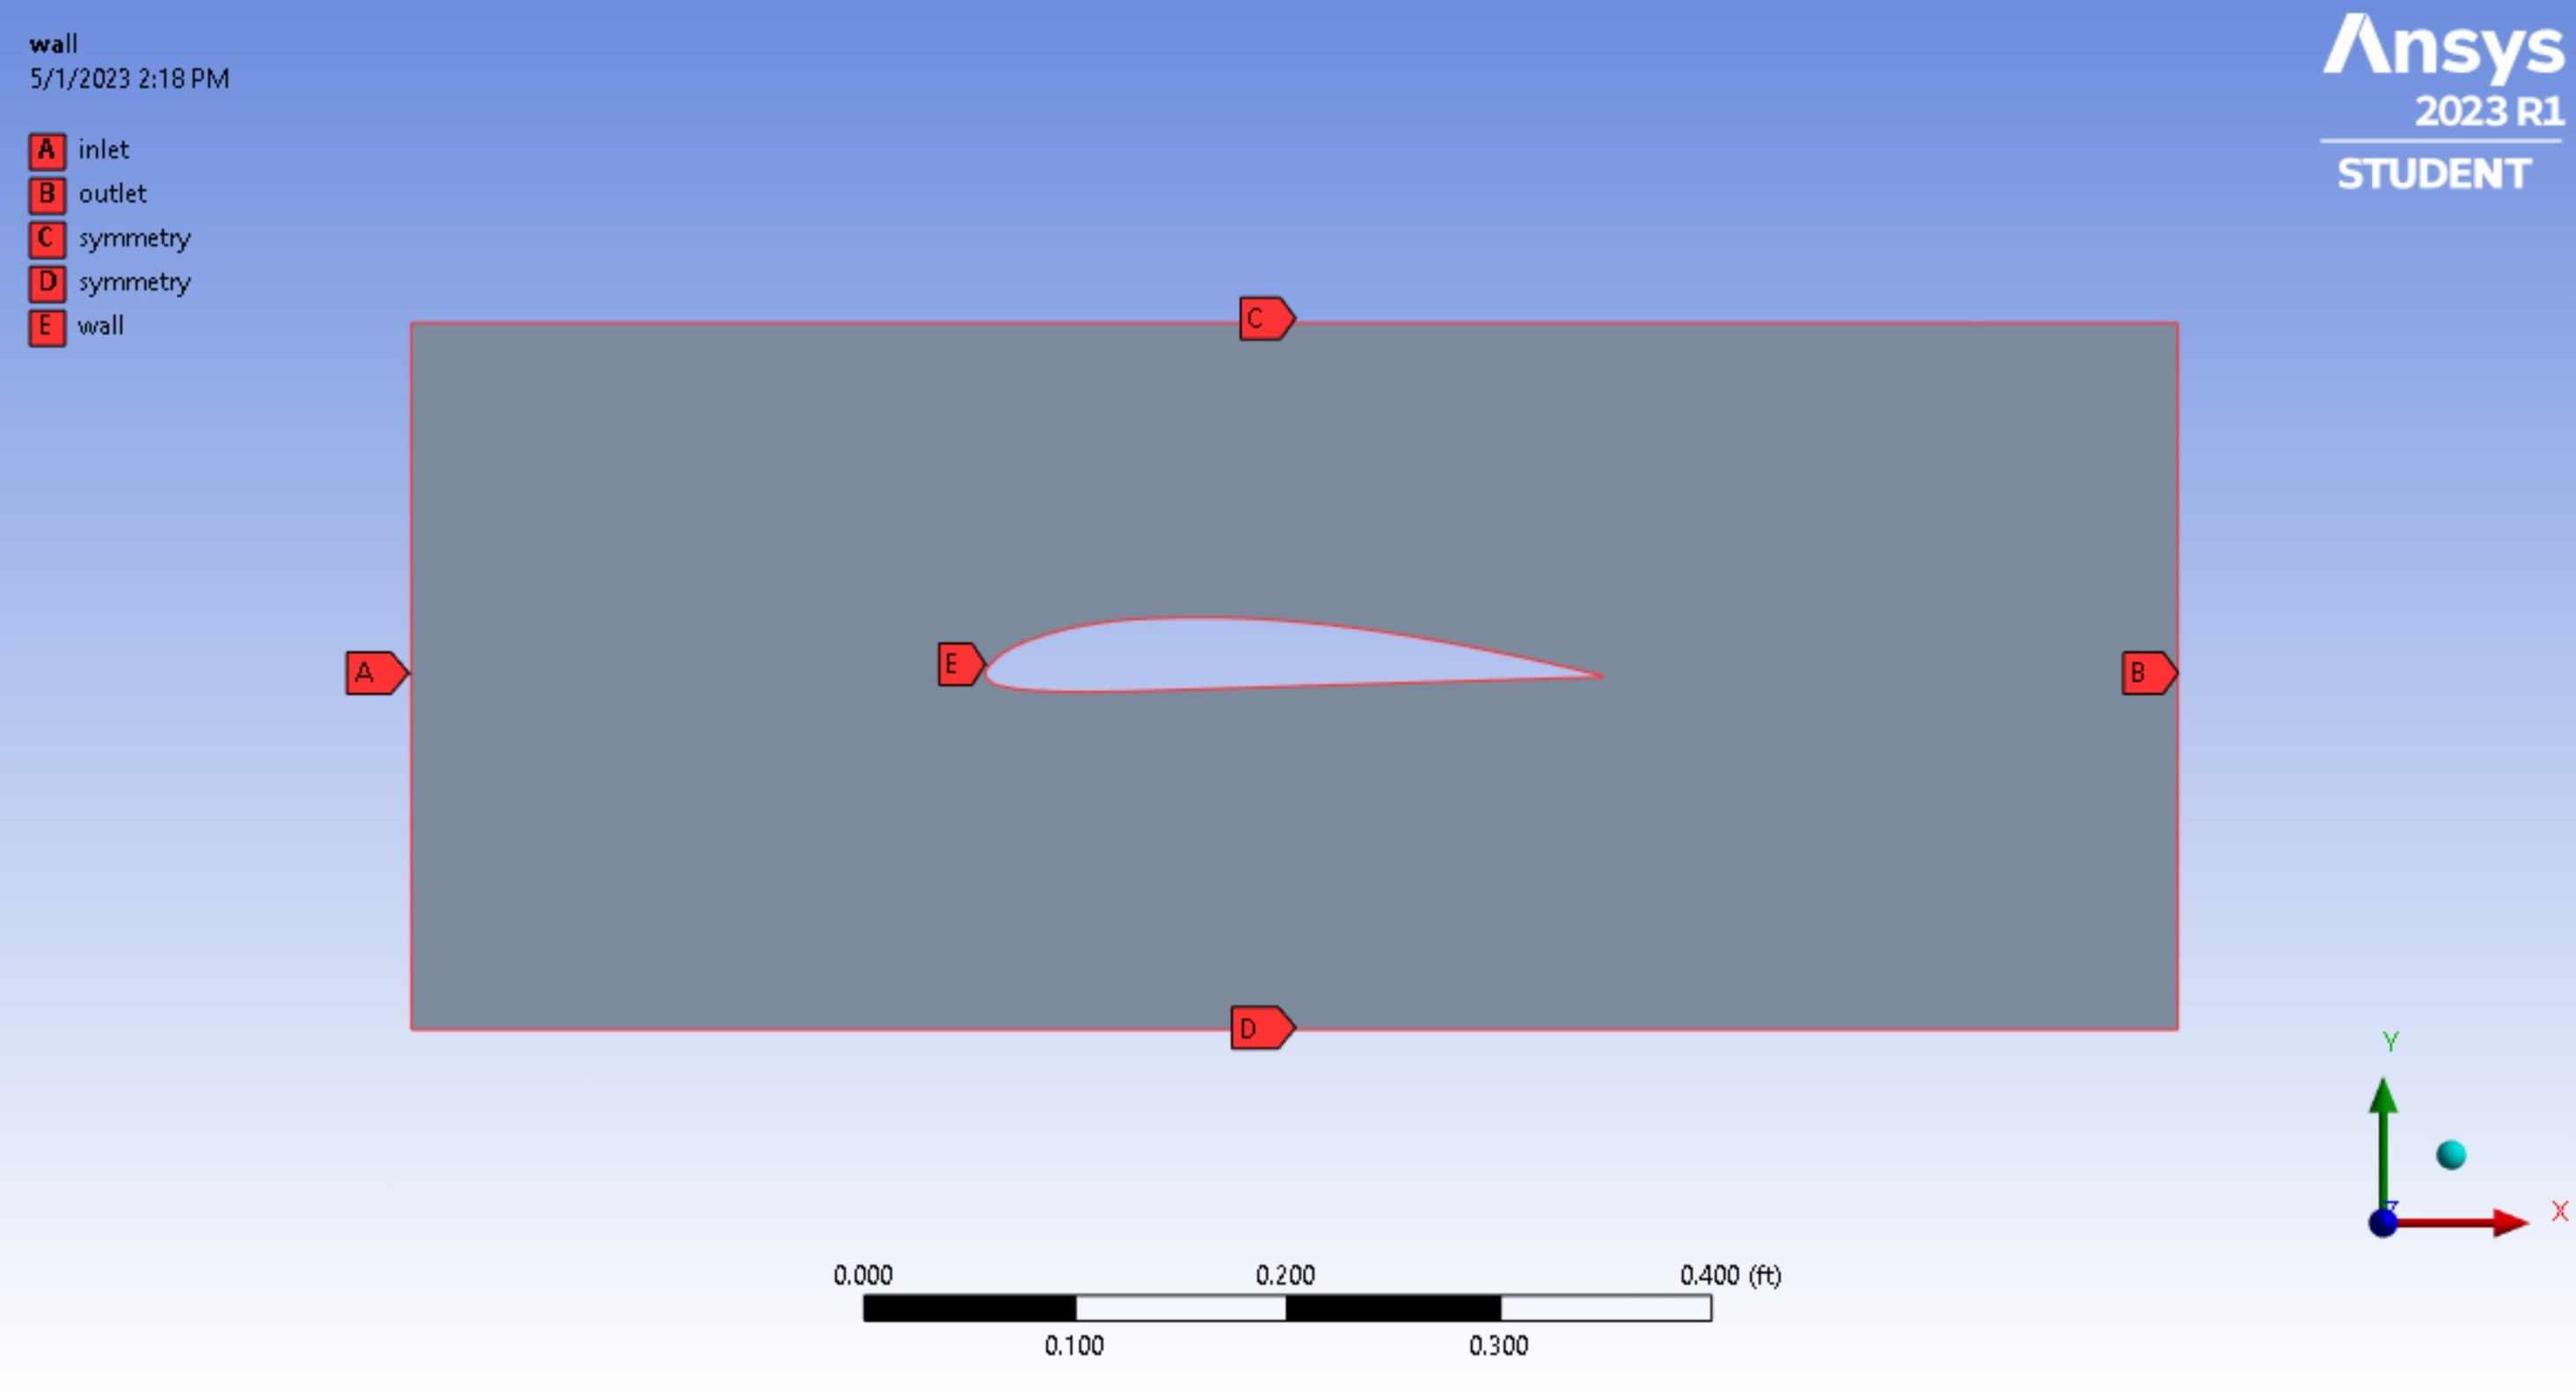
\includegraphics[width=15cm]{figures/BoudnaryConditionsFigure.jpg} }}% 
    \caption{A figure of the Clark Y-14 Airfoil with the associated boundary conditions.}
    \label{fig:BC}%
\end{figure}  

\begin{figure}[H]% 
    \centering
    {{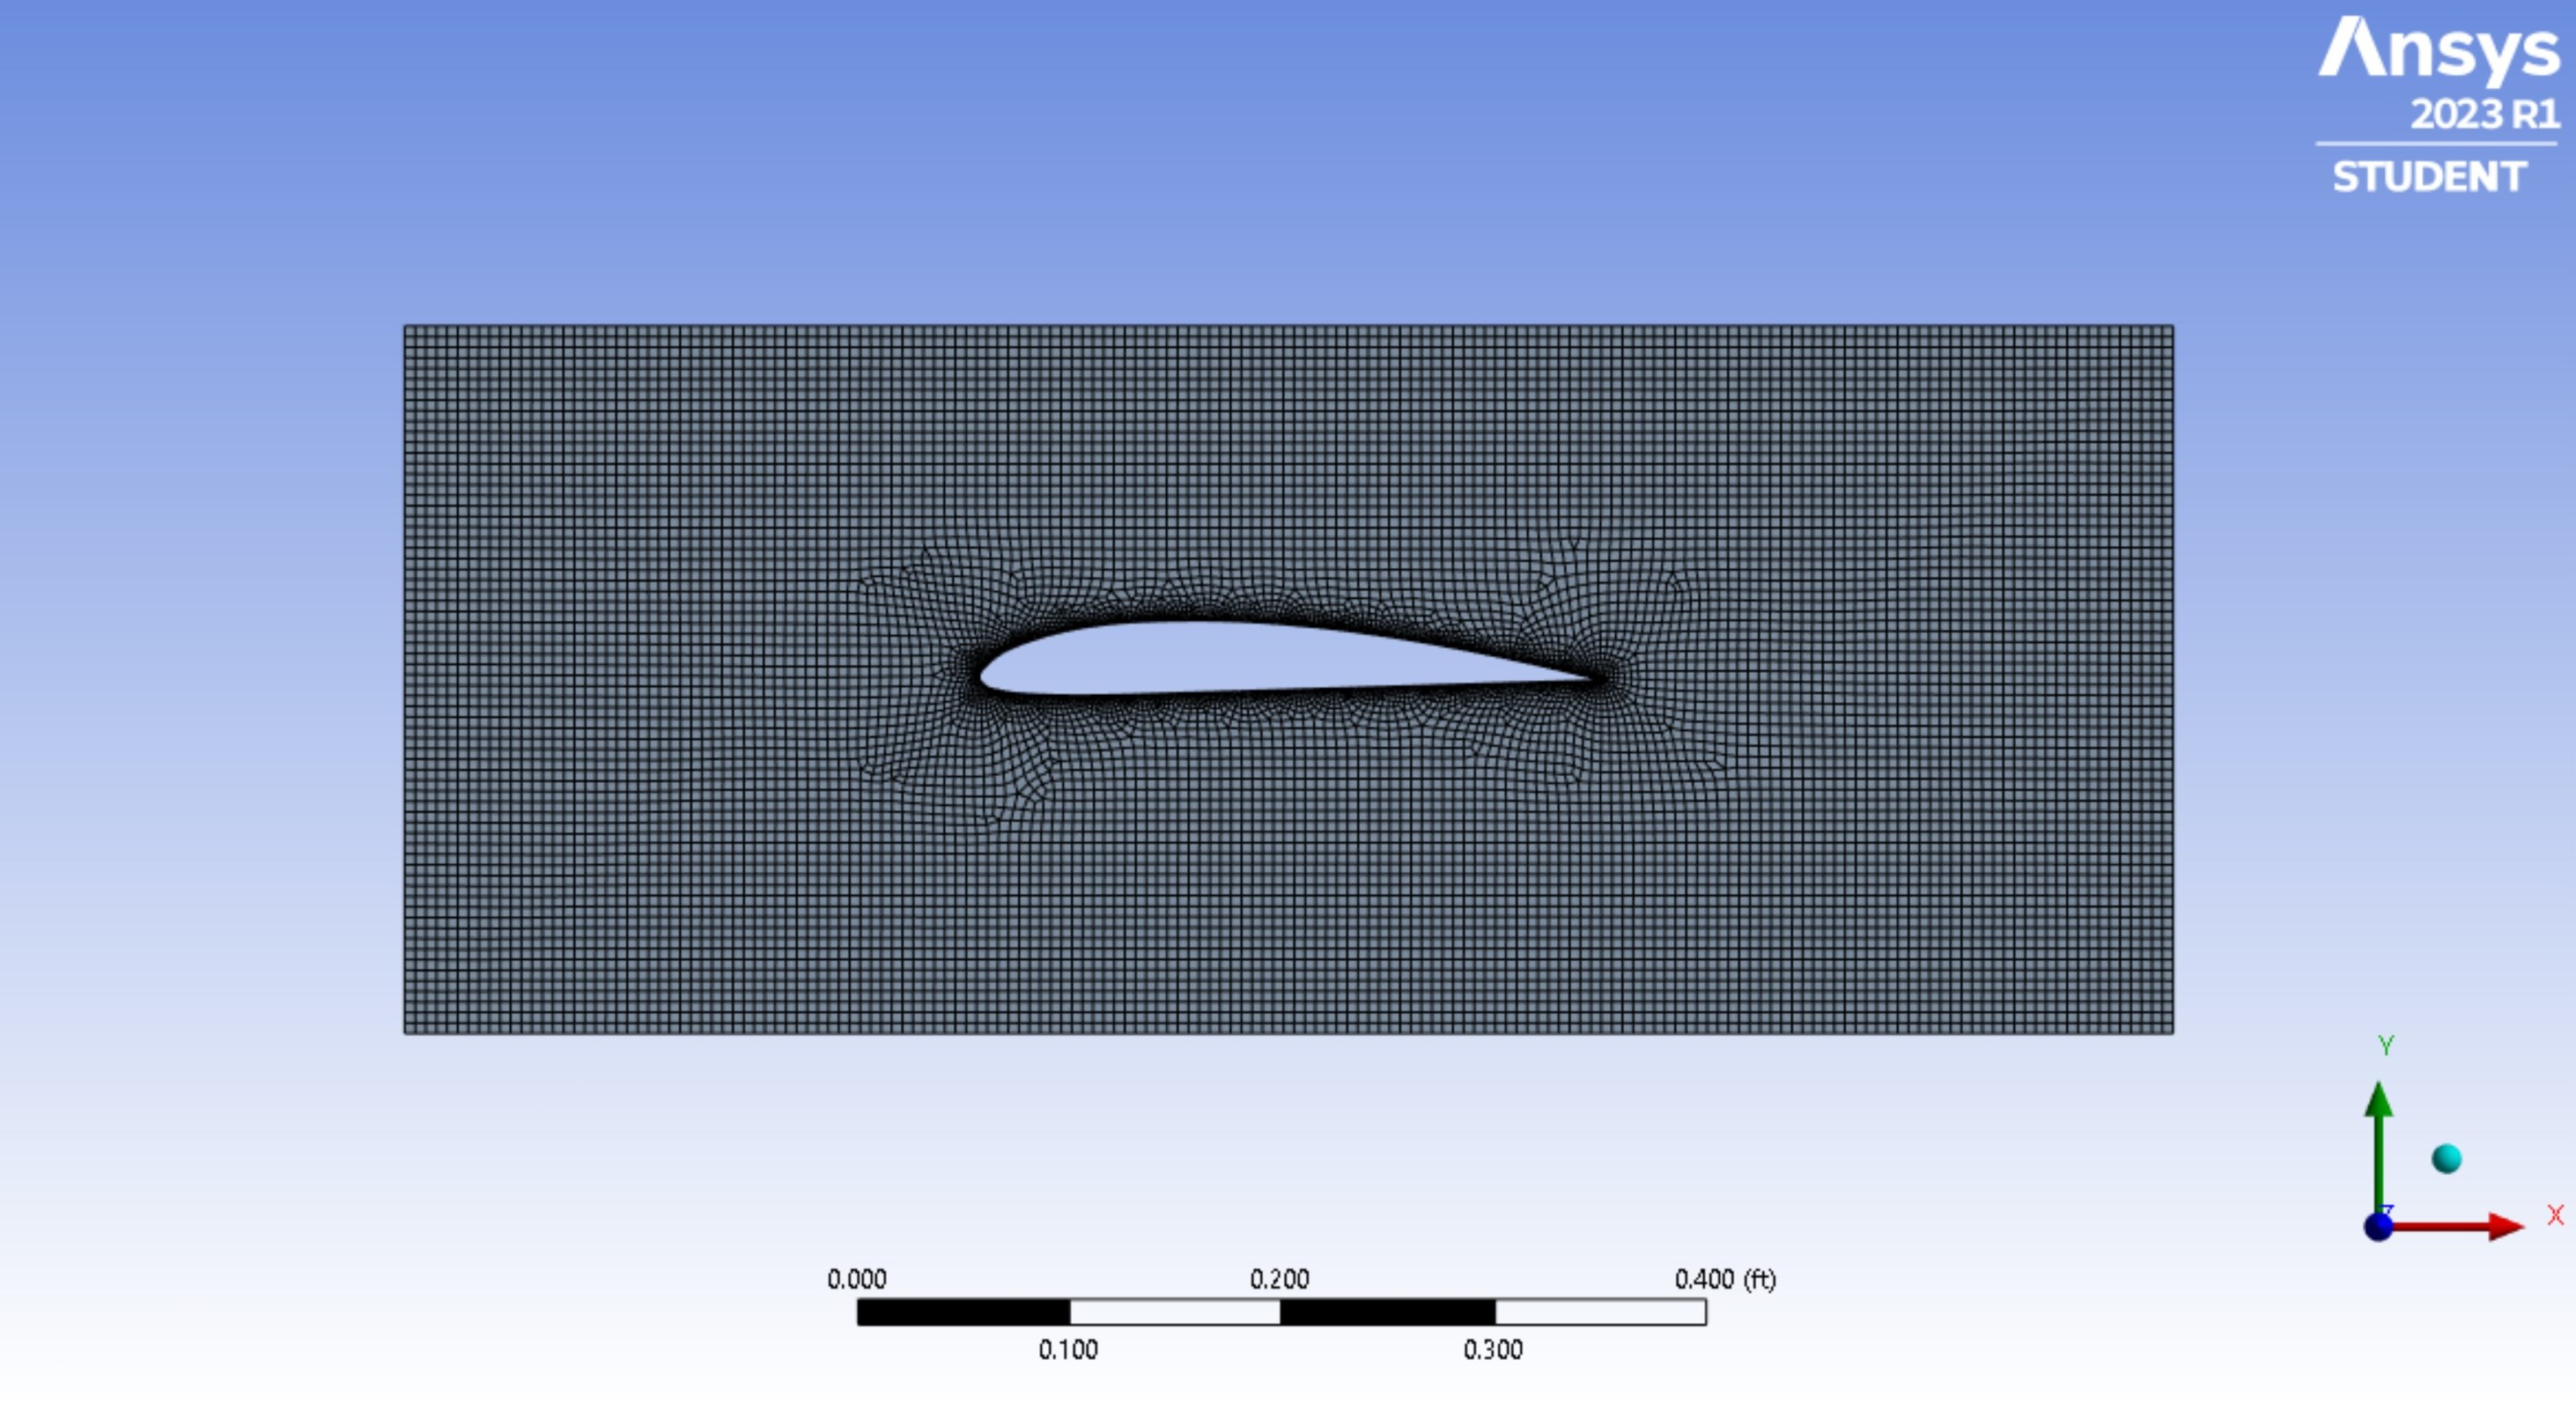
\includegraphics[width=15cm]{figures/MeshFigure.jpg} }}% 
    \caption{A figure of the mesh for the Clark Y-14 Airfoil.}
    \label{fig:Mesh}%
\end{figure}

Once the mesh was generated, the simulation solver was configured. A pressure-based, steady solver, using absolute velocity and planar 2D space was used in this simulation. As previously stated, the K-epsilon model was implemented in this simulation. Air was chosen as the working fluid. The inlet was defined as "velocity inlet" and the velocities were varied between 40 mph and 200 mph. The outlet was defined as a pressure-based outlet at 0 kPa. Under the Solution Methods tab, the Momentum, Turbulent Kinetic Energy, and Turbulent Dissipation Rate were all set to "Second Order Upwind." The pseudo-time method was set to Global Time Step. The simulation was initialized with a standard initialization. Lastly, the number of iterations was set to 500. 

%5 
\section{Results}
\begin{comment}
A well-organized and objective presentation of the results should be given. Not only the results, but also
the method of computation or derivation used to obtain them should be presented unless it is described
in another section, for example, ”Procedure”. If the method is involved, one complete example may be
included; however, if this example entails a lengthy computation or derivation, it may be put in appendix
and only the main steps indicated under ”Results”.
Tables and figures that show the results should be referred to in this section. A tabular form for the results
is more useful if many readers might want to plot the results in a variety of forms; graphs are preferable
in showing trends and comparisons. All statements about the results and any numerical values cited from
them should agree precisely with tables and figures.
In short papers the presentation of results may be combined with other sections, such as ”Procedure” or
”Discussion”. The heading should be altered accordingly, for example, ”Results and Discussion”.
\end{comment}

\subsection{Project Objective 1}
% plots outlined in the Objective 1 section of the assignment description. results for C_D and C_L for wind tunnel and CFD. 
Data from the wind tunnel experiment was recorded by nine different groups. Each group measured the manometer water height with respect to the atmospheric manometer for two velocities at different angles of attack. Each measurement was repeated by at least two groups. The data was combined into a single file and converted into meters and results for the same experimental conditions were averaged together.
\par
\bigskip

Using the Julia Programming Language \cite{bezanson2017julia}, an algorithm was written to integrate the pressure with respect to the horizontal distance between ports. This produced the force per unit length of the wing. The ports did not reach to the end of the airfoil so the pressures at the endpoints were estimated using linear extrapolation. Since the experimental data is discrete, the trapezoid rule, Equation (\ref{Eq:trap}), was used to numerically approximate this integral. Using the sum of the force on the top and bottom of the airfoil, the net force normal to the top of the airfoil per unit length was determined. Then, using the angle of attack, the force vector was projected onto the vertical axis to determine the lift force. \\


\begin{equation}
    \sum_{n=1}^{n_p} \frac{1}{2}(y(x_{n+1}) + y(x_{n}))(x_{n+1}-x_n)
    \label{Eq:trap}
\end{equation} \\



\noindent Since density, velocity, planform area, and the lift force were then known, the coefficient of lift can be found using the following: 

\begin{equation}
    C_L = \frac{2 F_L}{\rho g V^2 A}
    \label{Eq:C_L}
\end{equation}

\par
\bigskip
The Coefficients of Lift calculated from the wind tunnel experiment were plotted over the CFD data for Reynolds numbers of $1.09\cross10^5$ and $1.77\cross10^5$ in Figure (\ref{fig:C_L_vs_alpha_Wt_CFD}). The plot of Coefficient of Lift vs the angle of attack for the wind tunnel data is shown in Figure (\ref{fig:C_L_vs_alpha_Wt}). The plots for $C_L$ vs. $\alpha$, $C_D$ vs. $\alpha$, $\frac{C_L}{C_D}$ vs. $\alpha$, and $C_L$ vs. $C_D$ are show in Figures (\ref{fig:C_L_vs_alpha_CFD}), (\ref{fig:C_D_vs_alpha}), (\ref{fig:C_L_C_D_vs_alpha}), and (\ref{fig:C_L_vs_C_D}). 

%These height differences were used to calculate the gauge pressure at each orifice. The pressure difference over the wing was determined by integrating the pressures over the wing geometry. This pressure difference was then used to calculate the lift force. The lift force is then used in Equation (\ref{eq:C_L}) to find $C_L$.


%\begin{equation}
%    C_{L} = \frac{F_{L}} {2 \rho V^2 A} 
%    \label{eq:C_L} \\
%\end{equation}



\begin{figure}[H]% 
    \centering
    {{\includesvg[width=15cm]{figures/C_L_vs_alpha_Wt_CFD.svg} }}% 
    \caption{Plot of Coefficient of Lift vs. $\alpha$ data from the wind tunnel experiment and CFD for Reynolds numbers of 1.09E5 and 1.77E5.}
    \label{fig:C_L_vs_alpha_Wt_CFD}%
\end{figure}  

\begin{figure}[H]% 
    \centering
    {{\includesvg[width=15cm]{figures/C_L_vs_alpha_wt.svg} }}% 
    \caption{Plot of $C_L$ vs. $\alpha$ data from the wind tunnel experiment.}
    \label{fig:C_L_vs_alpha_Wt}%
\end{figure}  

\begin{figure}[H]% 
    \centering
    {{\includesvg[width=15cm]{figures/C_L_vs_alpha_CFD.svg} }}% 
    \caption{Plot of $C_L$ vs. $\alpha$ data from the CFD simulation.}
    \label{fig:C_L_vs_alpha_CFD}%
\end{figure}  

\begin{figure}[H]% 
    \centering
    {{\includesvg[width=15cm]{figures/C_D_vs_alpha.svg} }}% 
    \caption{Plot of $C_D$ vs. $\alpha$ data from the CFD simulation.}
    \label{fig:C_D_vs_alpha}%
\end{figure}  

\begin{figure}[H]% 
    \centering
    {{\includesvg[width=15cm]{figures/C_L_C_D_vs_alpha.svg} }}% 
    \caption{Plot of $\frac{C_L}{C_D}$ vs. $\alpha$ data from the CFD simulation.}
    \label{fig:C_L_C_D_vs_alpha}%
\end{figure}  

\begin{figure}[H]% 
    \centering
    {{\includesvg[width=15cm]{figures/C_L_vs_C_D.svg} }}% 
    \caption{Plot of $C_L$ vs. $C_D$ data from the CFD simulation.}
    \label{fig:C_L_vs_C_D}%
\end{figure}  


\subsection{Project Objective 2}
In order to determine the minimum runway distance required for the airplane to safely takeoff and land, the distance required for landing was calculated and compared with the minimum distance for take off. This system in the liftoff case can be seen in the following Free Body Diagram:

\begin{figure}[ht!]
    \centering
    {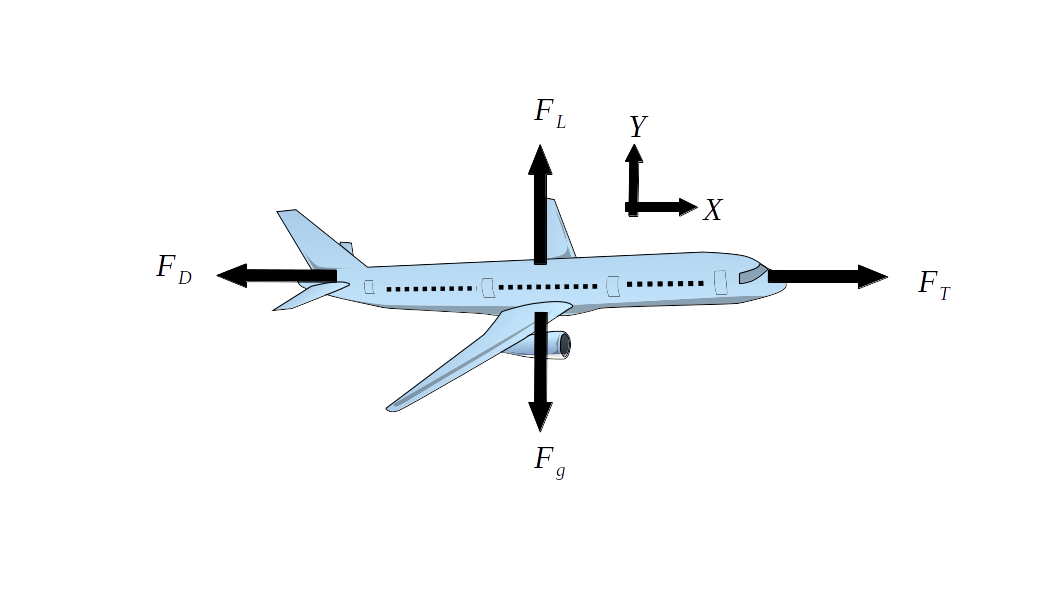
\includegraphics[width=10cm]{figures/fbd_1.png}}% 
    \caption{Free Body Diagram of the plane during liftoff.}
    \label{fig:liftoff}
\end{figure}  

\noindent To calculate the liftoff distance, the forces in the $y$-direction, as seen in Figure (\ref{fig:liftoff}), were equated:

\begin{equation}
    F_L = mg \\
    \label{Eq: yforces}
\end{equation}
\vspace{.5mm}

\noindent Substituting Equation (\ref{Eq: Lift}) into Equation (\ref{Eq: yforces}) and solving for velocity results in the following:\\

\begin{equation} \label{Eq: Lift}
    F_L = \frac{1}{2} C_L \rho g V^2 A
\end{equation} \\
\vspace{.5mm}

\begin{equation}
        V = \sqrt{\frac{2mg}{C_{L}\rho A}}
        \label{Eq: iterate_condition}
\end{equation}  \\

\noindent Because velocity and the Coefficient of Lift are dependent on each other, a recursive algorithm was used to find the velocity at which the wheels lift off of the ground. This algorithm was executed as follows: given an $\alpha$, pick a $C_L$. Find the velocity, $V_{guess}$, associated with this $C_L$. Substitute $C_L$ into Equation (\ref{Eq: iterate_condition}) and return $V_{check}$. If $V_{check} = V_{guess}$, return $V_{guess}, C_L$, and $C_D$. If $V_{check} \neq V_{guess}$, pick a new $C_L$ and restart the loop. In the case that none of the values for $C_L$ and $V_{guess}$ meet the return condition, use linear interpolation to find $C_L, V_{guess},$ and $C_D$ in between the CFD values.\\

\noindent Once $C_D$ and $V_L$ were found, we can create another Free Body Diagram considering the landing case.

\begin{figure}[ht!]
    \centering
    {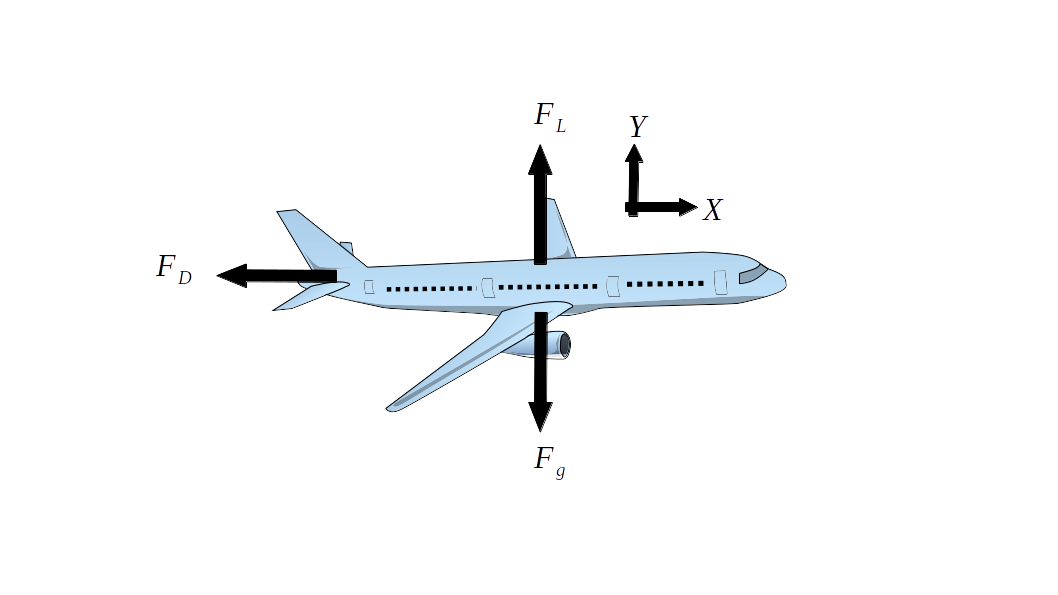
\includegraphics[width=10cm]{figures/fbd_2.png}}% 
    \caption{Free Body Diagram of the plane during landing.}
    \label{fig:landing}
\end{figure}  

\noindent The forces in the $x$-direction as seen in Figure (\ref{fig:landing}) were summed as follows: \\

\begin{equation}
    F_D = ma_x
    \label{Eq: I_don't_know}
\end{equation}\\

\noindent Substituting $\frac{1}{2} C_D \rho V^2 A$ for $F_D$ and solving for $a_x$ yields:\\

\begin{equation}
    a_x = \frac{C_D \rho V^2 A}{2 m}. \\
\end{equation}\\

\noindent Assuming that the drag force is constant during the whole landing, constant acceleration kinematic equations may be used. \\

\begin{equation}
    t = \frac{V_f - V_i}{a_x}. 
\end{equation}\\

\noindent Once the time it takes to land is calculated, $\Delta x$ can be found: \\

\begin{equation}
    \Delta x = V_i t + \frac{1}{2} a t^2v \\
    \label{Eq: dx_landing}
\end{equation}\\

\noindent In order to verify that the airplane can take off within this distance, the following calculations were done. First, the algorithm outlined above was used to find $C_{L,max}$, $V_{guess}$, and $C_D$. Using $C_D$, $F_D$ was solved for. Assuming it takes 30s to take off, $a_x$ was as follows:\\

\begin{equation}
    a_x = v_f/t
    \label{Eq: acceleration}
\end{equation}\\

\noindent The distance required for take off was found using Equation (\ref{Eq: dx_landing}). Lastly, summing the forces in the $x$-direction and solving for thrust yields:\\

\begin{equation}
    F_t = m a_x + F_D
    \label{Eq: Thrust}
\end{equation}  \\

Upon the completion of this process, we determined that the minimum runway length, with a safety factor of 1.25 applied, is $4640$ m and the maximum thrust is $113$ kN. 


\section{Discussion} 
\begin{comment}
Discussion of the results, together with their analysis, to show that the conclusions are warranted is one of
the most important parts of the paper. Each major conclusion should be clearly explained and comparisons
should be made with results of similar work by other investigators. If the results have an immediate applica-
tion, this should be pointed out in the discussion and, if possible, an example should be worked out to show
the method of application. All statements should be clear to readers who are in other fields of aeronautical
science and may not be so well acquainted with the subject as the author
\end{comment}
\noindent The wind tunnel and CFD data were similar in terms of the trends that they showed. The obsereved discrepancies can be attributed to many disperate factors. For example, it is possible that some groups may have misinterpreted their manometer readings and provided inaccurate data. Also, the wind tunnel data may be inconsistent because the data points had to be interpolated due to some manometer ports being incorrectly configured. Finally, error also resulted from the inability of the manometer to capture the effects of shear forces on the wind tunnel model. The Coefficient of Lift vs. $\alpha$ plot shows that the angle with the maximum Coefficient of Lift is $10^\circ$ for the wind tunnel and $15^\circ$ for the CFD. These values for $\alpha$ seem reasonable when compared with other airfoils. For example, the Clark Y airfoil has its maximum coefficient of lift at the $\alpha$ of $15^\circ$ \cite{clark_y_airfoil}.  
% Analysis of runway length and thrust and discussion on the reliability of our results. 
\par
\bigskip

\noindent The maximum thrust and minimum runway length results seem reasonable, given the assumptions, when compared with real-world examples. The Fokker 100 is similar in size to the one analyzed in the project, with a maximum takeoff mass of $45,810$ kg, a wingspan of $28.1$ m, and a wing area of $93.5$ m$^2$. The calculated maximum takeoff thrust was $112$ kN, whereas the thrust of the Fokker 100 engines can produce is $134$ kN. The calculated minimum runway length was $4640$m and the runway length for the Fokker 100 is $1,350$ m \cite{burger_2018}. Considering that these two planes are not identical, this error is within the bounds of reason. The error could also stem from all the assumptions and simplifications that were made. For example, one assumption is that the deceleration when landing is only affected by drag and is assumed to be constant. This assumption was used to simplify calculations and does not accurately represent what would happen in reality. Another simplification that does not reflect reality would be the Coefficient of Lift and the Coefficient of Drag being constant. These Coefficients would change as a function of the velocity. Finally, the plane is not utilizing landing gear brakes or brake flaps which would significantly impact the force of drag. This no doubt results in a longer runway. With this in mind, this project provides an initial approximation for a potential runway design.


\section{Acknowledgements}
We would like to thank Dr. Joseph Thalakkottor, Assisant Professor of Mechanical Engineering at South Dakota Mines, for his assistance in this project. Specifically, for setting up and providing the experimental equipment and correcting some of our errors and misconceptions during the research process.

\par
\bigskip

\newpage
\phantomsection   % 
\printbibliography[heading=bibintoc, title={References}]

\begin{comment}
\newpage
\section{Appendix}
\indent
\lipsum[1]
\end{comment}

\end{document}

